\documentclass[12pt]{article}
\usepackage{amsmath}
\usepackage{amssymb}
\usepackage{amsthm}
\usepackage{accents}
\usepackage{graphicx}
\setlength{\oddsidemargin}{0in}
\setlength{\textwidth}{6.5in}
\setlength{\topmargin}{-.55in}
\setlength{\textheight}{9in}
\pagestyle{empty}
\renewcommand \d{\displaystyle}
\begin{document}
\noindent Dallas Klumpe

\noindent Math 5820

\noindent HW 16

11.2.1. Plot these data and find the equation of the least squares line, $y=a+bx$. Suppose a cricket of this species is observed to chirp eighteen times per second. What would be the estimated temperature?\\
\begin{center}
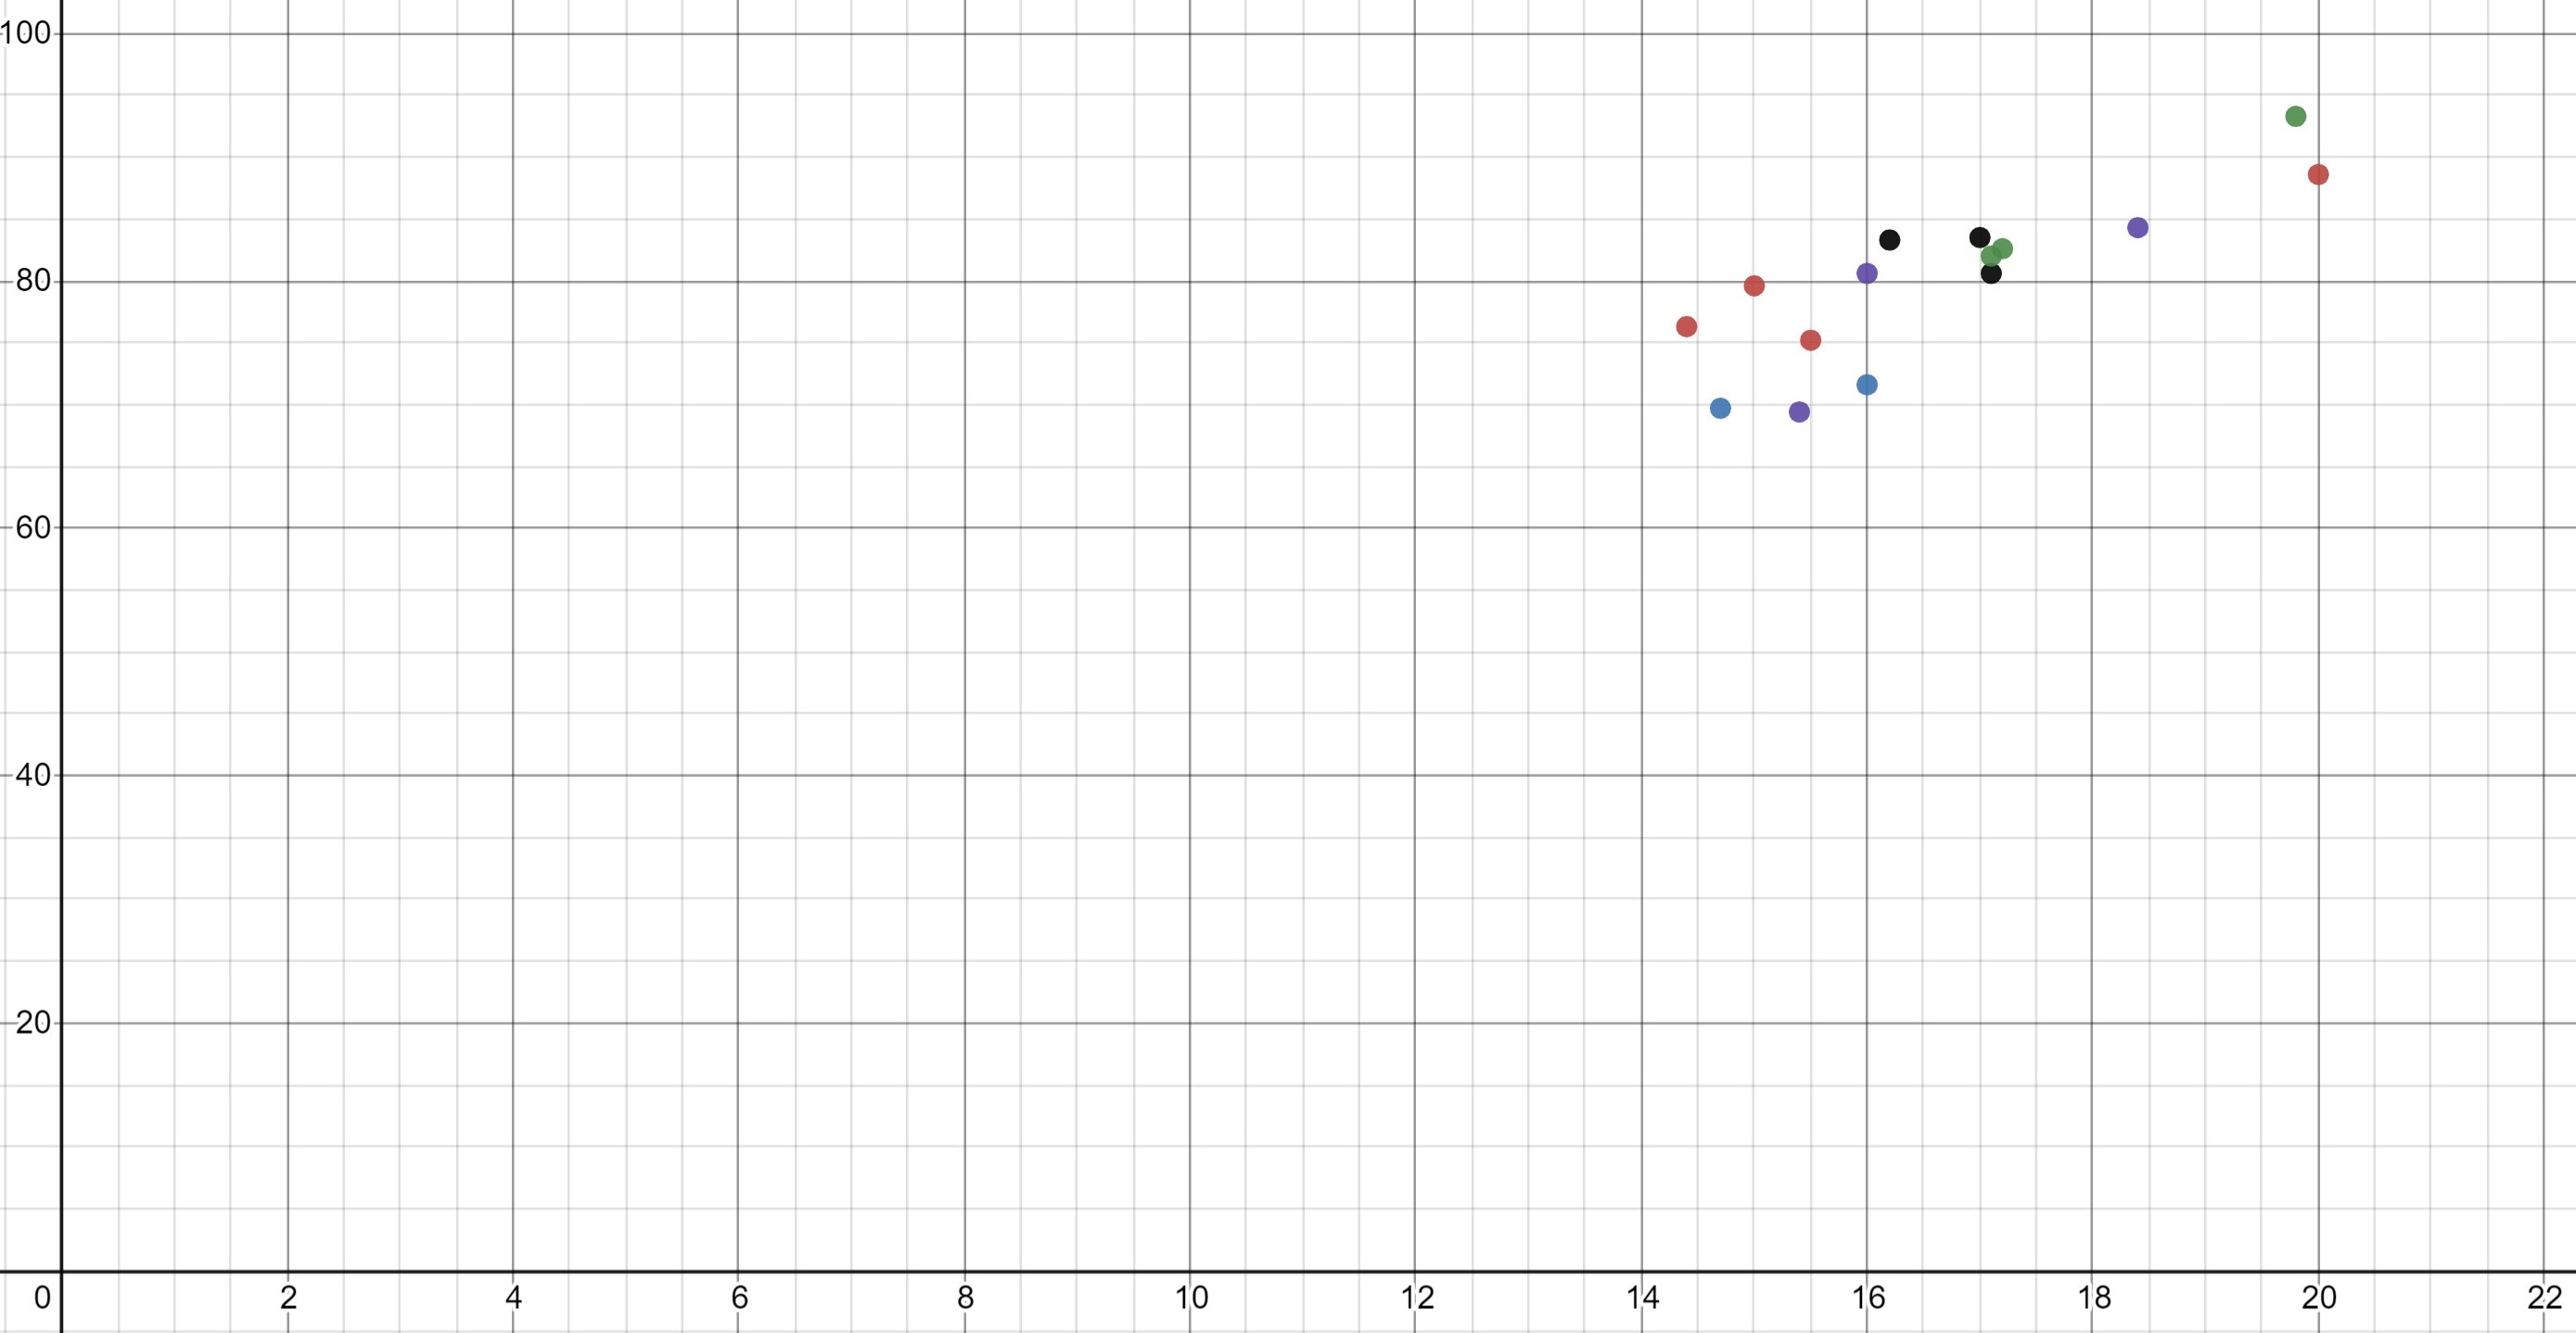
\includegraphics[scale=0.5]{11-2-1.JPG}
\end{center}
Well, given the sums, we have that $\beta_0=25.2323$ and $\beta_1=3.2911$ by Cramer's Rule. So, we have the least squares line $y=25.2323+3.2911x$. So, at $18$ chirps per second, we would expect the tempurature to be $84.47$ degrees fahrenheit.\\[20pt]

11.2.3. Calculate the residuals, $y_1-\hat{y}_1,\ldots, y_9-\hat{y}_9$, and draw the residual plot. Does it suggest that fitting a straight line through these data would be appropriate?\\
By the given data and the sums, we have that $\beta_0=67.5078$ and $\beta_1=0.8706$. So, $\hat{y}=67.5078+0.8706x$. Hence, $y_1-\hat{y}_1=-0.8078, y_2-\hat{y}_2=0.0098, y_3-\hat{y}_3=0.0862, y_4-\hat{y}_4=0.0332, y_5-\hat{y}_5=-0.0904, y_6-\hat{y}_6=0.1448, y_7-\hat{y}_7=0.5506, y_8-\hat{y}_8=1.6916$, and $y_9-\hat{y}_9=-1.6086$. Based on the residuals, a straight line would appear to fit the data.
\begin{center}
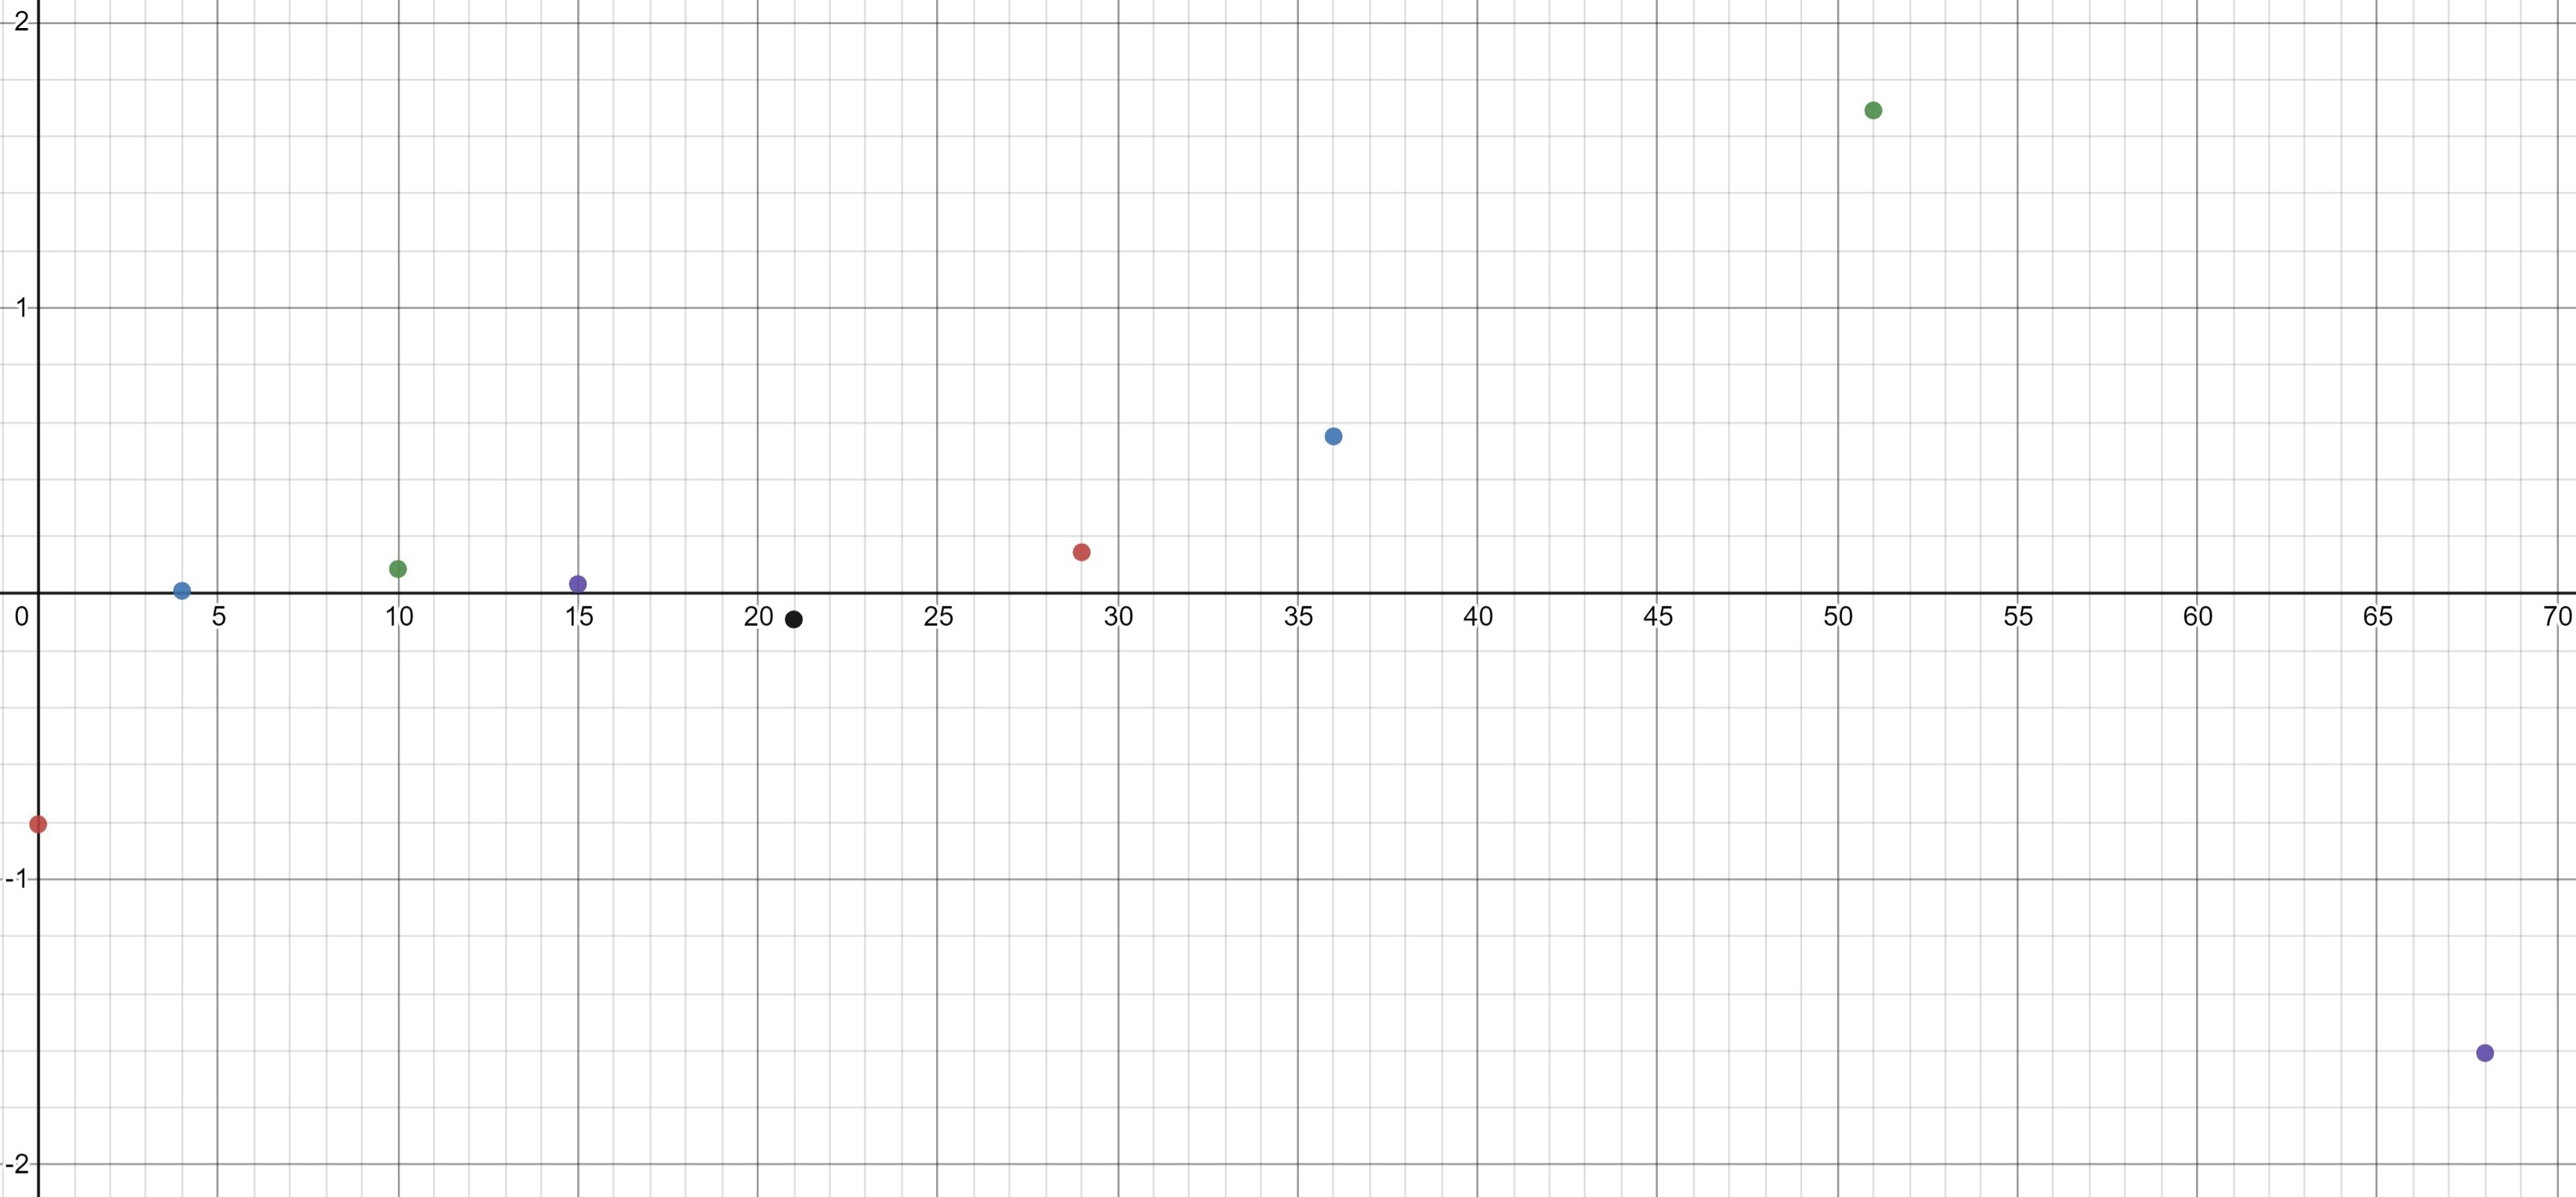
\includegraphics[scale=0.5]{11-2-3.JPG}
\end{center}

11.2.4. What, if anything, is unusual about the following residual plots?\\
Well, the residuals in the first plot are all positive, so there may be a pattern. The residuals in the second plot alternate from positive to negative with each $x-$value, indicating a pattern. So, from both of the residual data plots, and the possible patterns, we can conclude that a straight line would likely not fit the data for both of them.\\[20pt]

11.2.5. The following is the residual plot that results from fitting the equation $y=6.0+2.0x$ to a set of $n=10$ points. What, if anything, would be wrong with predicting that $y$ will equal 30.0 when $x=12$?\\
Well, the value $x=12$ is outside of the observed data on the residual plot, so we can't say whether or not the residuals continue to be random past about $x=8.5$. That is we cannot say for certain that $(12,30)$ would be an appropriate fit for the data.




\end{document}